

%%%%%%%%%%%%%%%%%%%%%%%%%%%%%%%%%%%%%%%%%%%%%%%%%%%%%%%%%%
\section{Using Biases}
\label{sec:usingbiases}
%%%%%%%%%%%%%%%%%%%%%%%%%%%%%%%%%%%%%%%%%%%%%%%%%%%%%%%%%%

This section makes use of an improved central bias model and the \textit{saccadic flow} model (described in Section \ref{ModellingFlow}). The new central bias model is similar to the model presented by \cite{clarke-tatler2014}, except for using a truncated Gaussian distribution to take the image boundaries into account. We present three examples of how these bias models can be used as priors in order to weight fixations, based on the fact that Flow produces likelihoods for any given fixation given the current fixation. First of all, we will demonstrate how we can weight fixations in gaze landscapes (also known as hotspot maps or heatmaps) to reduce noise and to give an improved visualisation of the image regions participants looked at more than expected. Secondly, we examine whether saccadic flow can be used to better understand the contribution of low-level features on fixation selection, and potentially lead to better evaluation of such computational saliency models. Finally, we demonstrate how flow can be used to generate a series of saccades, and compare these to observed human saccades. Being able to generate realistic synthetic datasets is useful to create an image-independent baseline with which to examine spatial maps of prediction using signal detection theory \citep[see][]{clarke-tatler2014}.

\subsection{Gaze landscapes}

One technique that is commonly used to visualise the spatial allocation of gaze is to create 'heatmap' plots where colour or luminance is used to indicate the density of fixation on those locations (Figure ~\ref{fig:adjustedHeatmaps}, column 2). A potential problem with visualising data in this way is that such maps represent all fixations as being of equal importance. For example, a location that is fixated for one second would be weighted equally with fixations that lasted half that time. If we want to make an assumption that fixation duration is intimately linked with the importance of that fixation (i.e. we will look longer at more informative information) then we can change our visualisation to weight fixations by their duration (Figure ~\ref{fig:adjustedHeatmaps}, column 3). \textbf{However, this weighted heatmap still fails to distinguish fixation behaviour likely to arise from image independent biases like the central fixation bias from fixation behaviour likely to reflect meaningful interrogation of, and response to, the viewed content.} 

\begin{figure*}
\centering
\includegraphics[width=13cm]{figs/heatmap_figure.png}
\caption{Examples of fixation heatmap plots from \cite{clarke2013}. The same fixations are presented where the Gaussian at each fixation is weighted by the duration of the fixation, the centre bias model from \cite{clarke-tatler2014} , and the saccadic flow model presented in this paper.}
\label{fig:adjustedHeatmaps}
\end{figure*}

An advantage of the \citet{clarke-tatler2014} model and the saccadic flow model presented here, is that we can represent fixations by the likelihood that they would occur based on the predictions of the models. Because the models reflect image-independent behavioural and oculomotor biases, fixations not predicted by these models might involve more high-level mechanisms. For example, given a tendency to fixate in the centre of the scene, we might consider saccades to non-central locations to be less predicted and therefore more likely to be image- or task-related.  In Figure ~\ref{fig:adjustedHeatmaps} (column 4 and 5) we present some overlaid heatmap data from the \citet{clarke2013} dataset, where fixations are weighted by the inverse probability of them occurring based on the models of central bias and saccadic flow. These figures reveal that representing data in this manner can allow us to visualise information that was important enough to disrupt these biases. In other words, these visualisations  remove some of the image-independent biases, and reveal the more important image \emph{dependent} information.


The top row of Figure ~\ref{fig:adjustedHeatmaps} demonstrates that weighting the fixations by the central bias and flow model both reduce the \emph{importance} of some fixations. The central bias model punishes fixations near the center of the image, while the flow model punishes fixations that were well predicted by the oculomotor biases of the saccadic flow model. Conversely, the models reward unlikely fixations. The second row reveals an instance of where the car to the left received less fixations than the pub sign, but that these fixations are boosted in the central bias and saccadic flow models where 'unlikely' saccades were made to this location. In the third and fourth rows, there are examples of images with important content near the centre of the photograph. This illustrates how the central bias model can sometimes over-compensate and reduce the influence of fixations in the centre of pictures that have important content located there. Given the tendency for photographers to centre their photographs around important content, reducing the weight of fixations to the castle in the painting (row 3) and the girl's face (row 4) would perhaps overly punish centrally biased photographic composition. With the flow model, however, these areas are still represented, as observers made saccades to theses regions that were unlikely to be driven by behavioural biases.

\subsection{Removing biases when examining image-dependent information}

By considering saccades in light of the probability that they were generated by image-independent biases, we can gain further insights into the image-dependent features that are important in attracting fixation. One feature that has been shown to correlate with fixation is visual salience \citep{parkhurst2002}. However, others have argued that this tendency is driven by the correlation between salient objects and their semantic interest \citep{henderson2007}, with interesting objects tending to be placed near to the centre of photographs \citep{tatler2007}. Oculomotor biases which favour a central tendency would predict the same fixation placement regardless of the distribution of salient objects in the image \citep{tatler-vincent2009}. Here, we can examine this question by looking at the relationship between saccade probability and the ability of different conspicuity maps to predict fixation. We can therefore examine how the effect of visual salience observed in eye movement analysis is related to the behavioural biases of eye movements.

We compared the proportion of fixations that fell in the brightest 20\% of pixels for salience maps to the likelihood of fixations from the flow and central bias models. Fixations were separated for each image into bins of 5\% from the least-likely to the most-likely to be generated based on salience. We then examined what proportion of each of these bins were in the brightest 20\% of salience maps using the Adaptive Whitening Saliency (AWS; \cite{garciadiaz2012}), RARE \citep{riche2013} and Graph-based visual saliency \citep[GBVS;][]{harel2006} algorithms. We selected AWS and RARE as they are the two best performing salience models according to the MIT Saliency Benchmark \citep{mit-saliency-benchmark,judd2012} with publicly available code, and GBVS as it contains a bias towards the centre cause by summing neighbouring pixel values across the spatial prediction map.

Figure ~\ref{fig:salmaps} reveals that the likelihood of making a saccade based on both the central bias and the flow model is highly related to salience in both AWS and RARE, with low-likelihood saccades being less likely to be to a salient region. Saccades that are very unlikely to be generated based on the oculomotor tendencies of eye movement (both flow and central bias) are therefore also less well explained by salience. Of the 5\% of fixations that were \textit{most} likely from saccadic flow, ~60\% of fixations fell in the 20\% thresholded region of the AWS map. However, of the 5\% of fixations that were \textit{least} likely from saccadic flow, only 40\% of fixations fell in this region. This means that it may be important to consider, and potentially remove, behavioural biases when attempting to predict fixation selection using feature-based models to ensure that any benefit in predictive power cannot be explained by behavioural biases correlating with salience. When examining a model that contains an inherent central bias (GBVS), we can see that weighting fixations by the \citet{clarke-tatler2014} central bias model is highly related to the performance of GBVS in predicting fixation selection.

%Examples of the maps can be seen in Figure \ref{fig:salmaps}. Salience maps were normalised to sum to 1, and data were analysed using linear mixed-effect models with the fixation weighting (duration, central bias or saccadic flow) as fixed effect factors, and image and participant as random effects. 

\begin{figure}
\centering
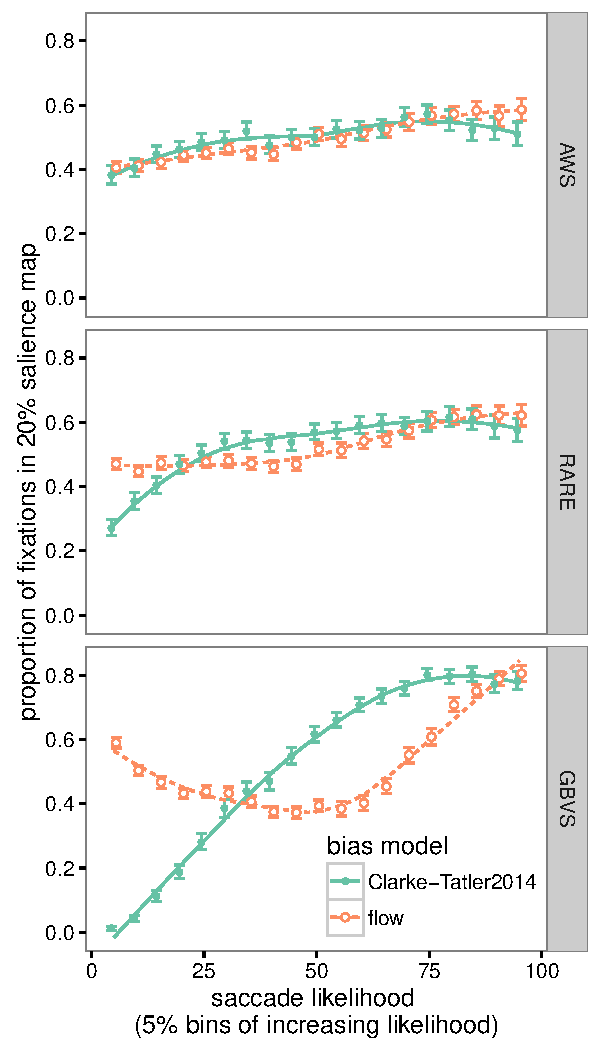
\includegraphics[width=\columnwidth]{figs/SaccadeSaliency.pdf}
\caption{Saccades binned by probability of them occurring in 5\% bins against the proportion of those fixations that fell in a 20\% thresholded region of AWS, RARE and GBVS salience maps.}
\label{fig:salmaps}
\end{figure}



\subsection{Saccadic Flow as a Generative Model}
\label{sec:humanComp}

Another use of the saccadic flow model is that it allows us to make spatial maps that relate to the probability of \emph{all saccades within a scene} based on the current position. For example, Figure~\ref{fig:flowPredict} shows that for three fixations in different locations within a scene, flow will make different spatial predictions of the next saccadic landing position. We can use this method to generate sequences of synthetic scan-paths. Here, we compare the distributions of these generated scan-paths with empirical scan-paths to determine which aspects of human saccadic behaviour are not captured by our model. To do this, we will create a merged dataset of fixations from the eight training datasets (175 000 fixations, including initial fixations, in total over 16 000 trials), and then generate a matched synthetic dataset such that the number of fixations in each trial is identical. 

\begin{figure*}[htb]
\centering
\subfigure[]{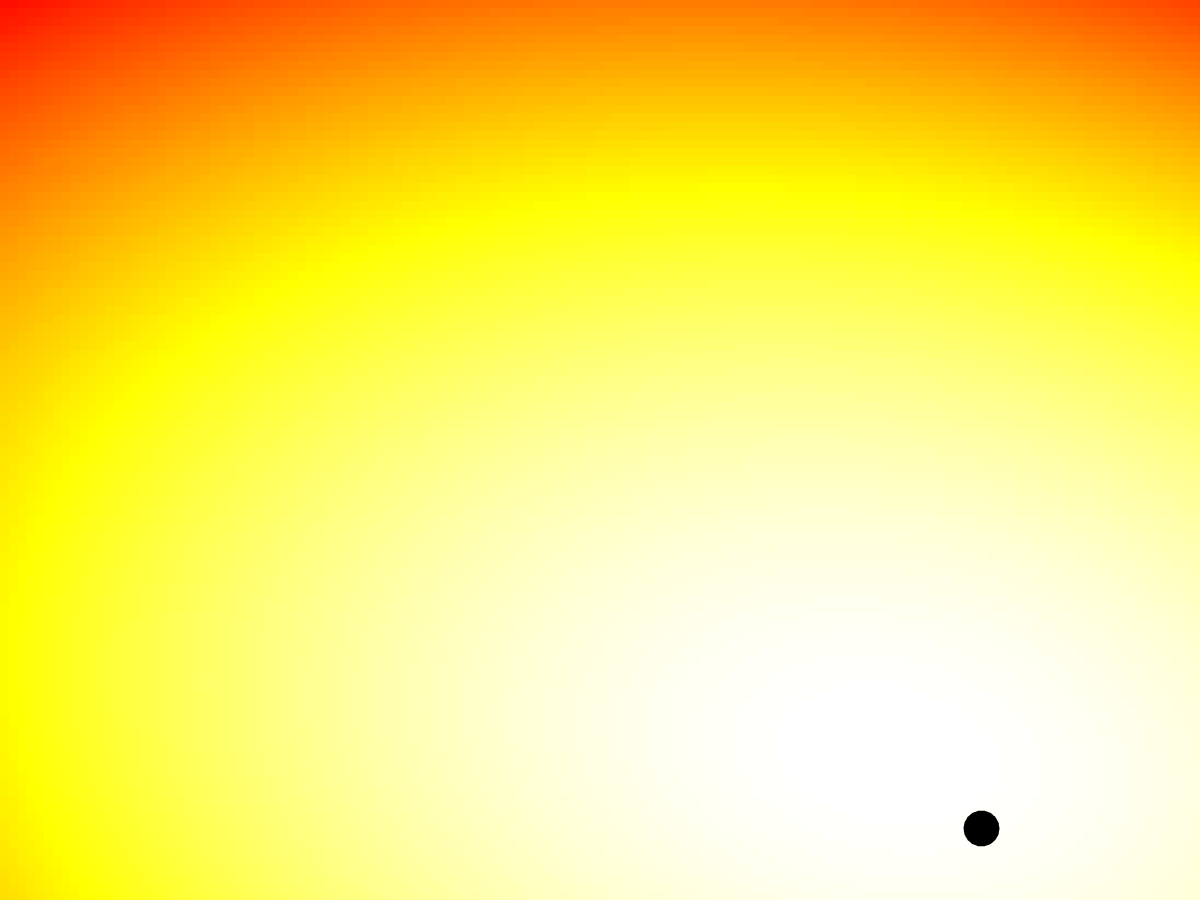
\includegraphics[width=4.2cm]{figs/DownLeft.png}}
\subfigure[]{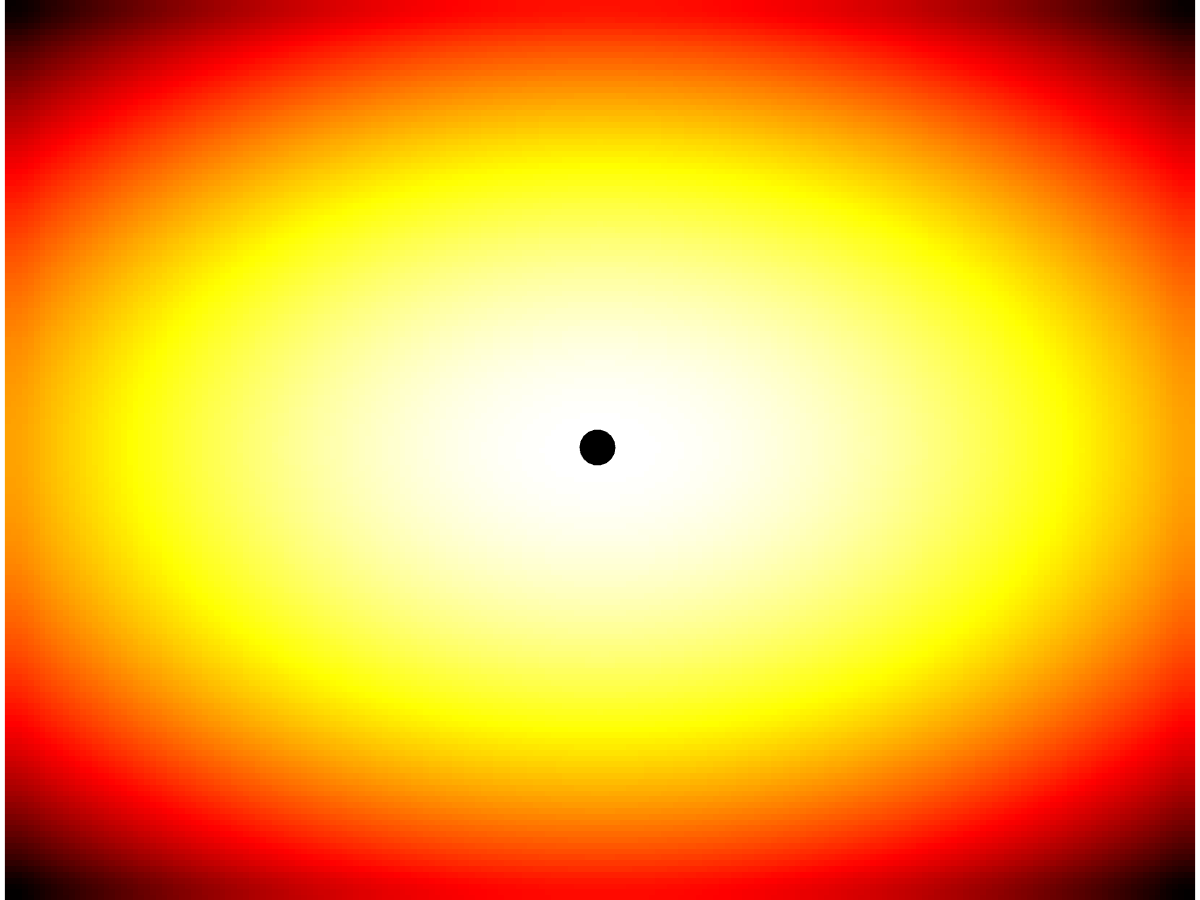
\includegraphics[width=4.2cm]{figs/Center.png}}
\subfigure[]{
\includegraphics[width=4.2cm]{figs/UpRight.png}}
\caption[]{Example spatial prediction maps for all potential saccade locations from 3 different fixation positions (black circles), to demonstrate how flow's predictions differ across the extent of a scene.}
\label{fig:flowPredict}
\end{figure*}

We can see from Figure \ref{fig:flowHumanComp}(a) and (b) that both the central bias and the saccadic flow model do a good job of capturing the distribution of fixation locations over the $x$ and $y$ axes. While it is not surprising that the central bias closely matches the empirical distributions (as this is exactly what it has been fitted to), it is interesting that saccadic flow does just as good a job. Hence, the central bias can be thought of as a property of saccadic flow, and does not need to be accounted for separately. 

When compared to the empirical distributions, both the central bias and saccadic flow appear to be slightly biased towards making fixations to the extreme edges of the image. This suggests that the truncated Gaussian distribution does not quite capture the effects of the image boundary on fixation selection and there is some additional aversion to fixating close to the screen edge. 

Another discrepancy between the synthetic and empirical distributions can be seen with saccadic amplitudes. While the flow model is a better fit to the human data than the central bias, it still underestimates the proportion of very short saccades (Figure \ref{fig:flowHumanComp}(c)). Interestingly, the flow model does manage to capture the initial increase in saccadic amplitudes after scene onset (Figure \ref{fig:flowHumanComp}(d)), but it does not explain the subsequent coarse-to-fine dynamics that are seen in the empirical scan-paths. 


\begin{figure}[htb]
\centering
\subfigure[]{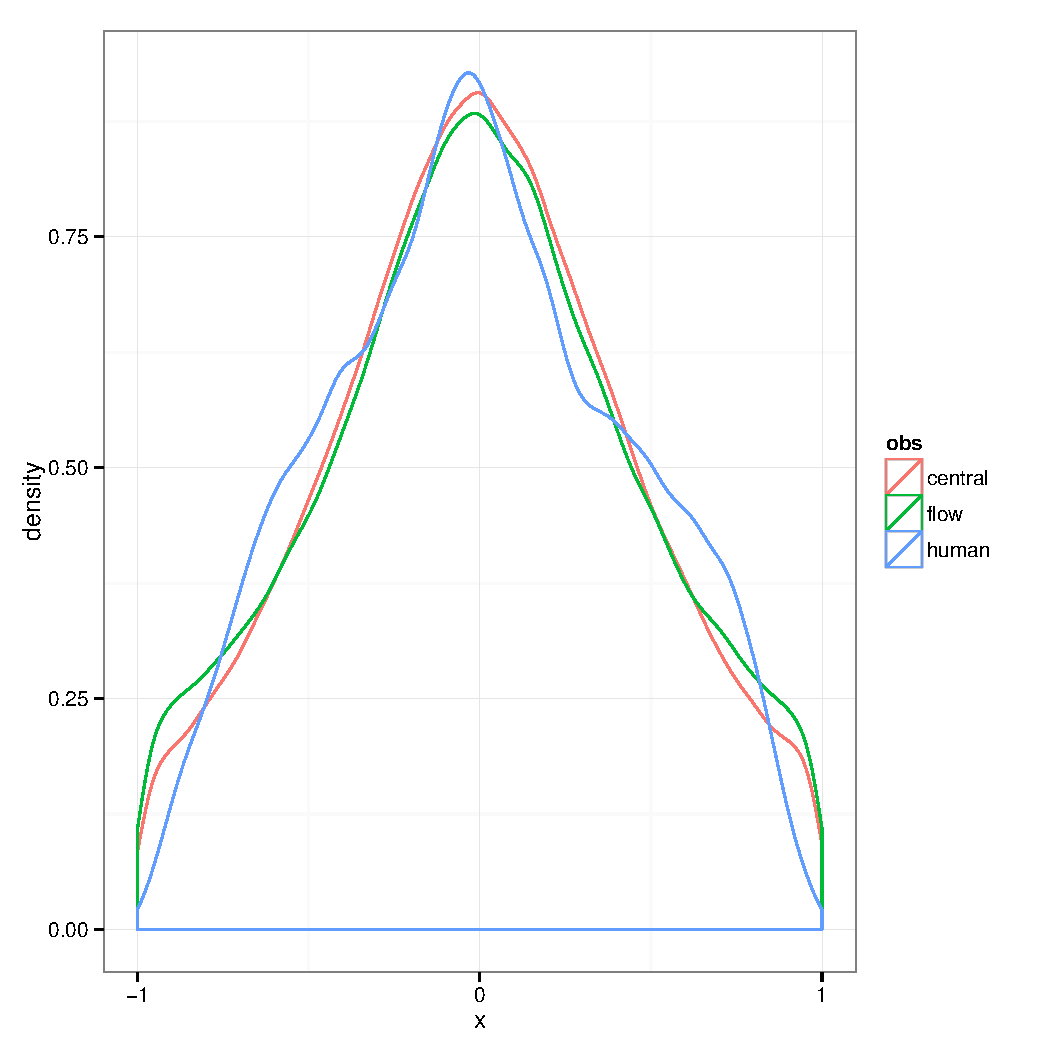
\includegraphics[width=3.8cm]{../scripts/coarse2fine/figs/xFixComparison}}
\subfigure[]{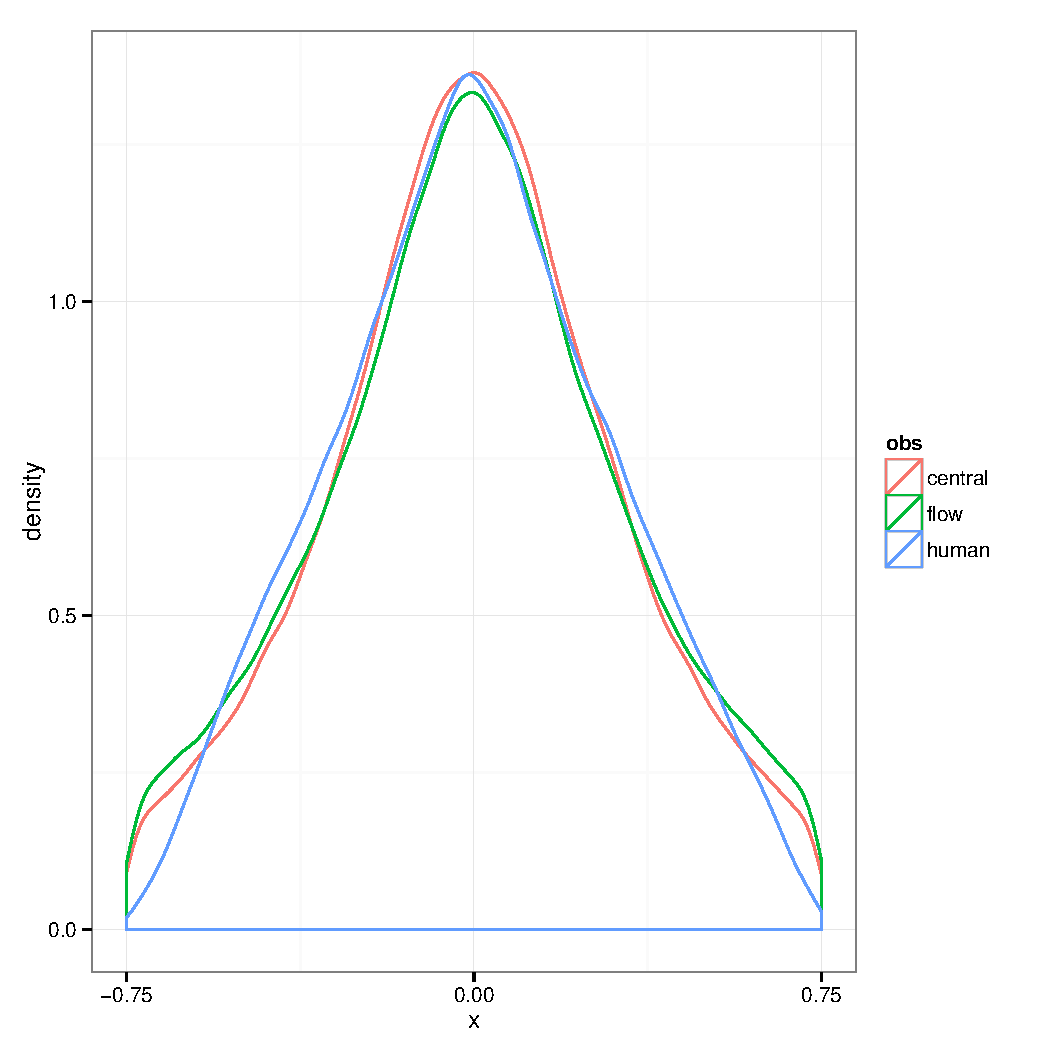
\includegraphics[width=3.8cm]{../scripts/coarse2fine/figs/yFixComparison}}
\subfigure[]{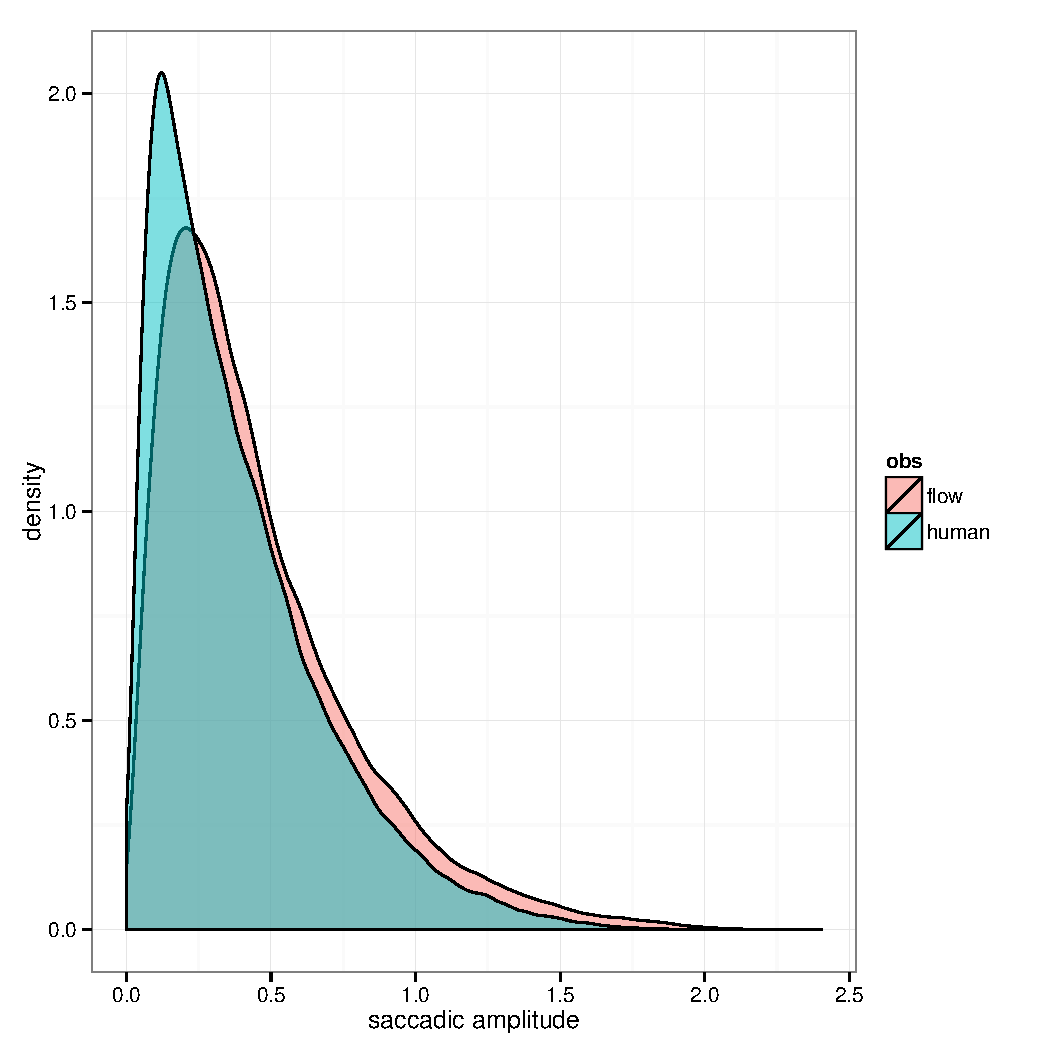
\includegraphics[width=3.8cm]{../scripts/coarse2fine/figs/ampSaccComparison}}
\subfigure[]{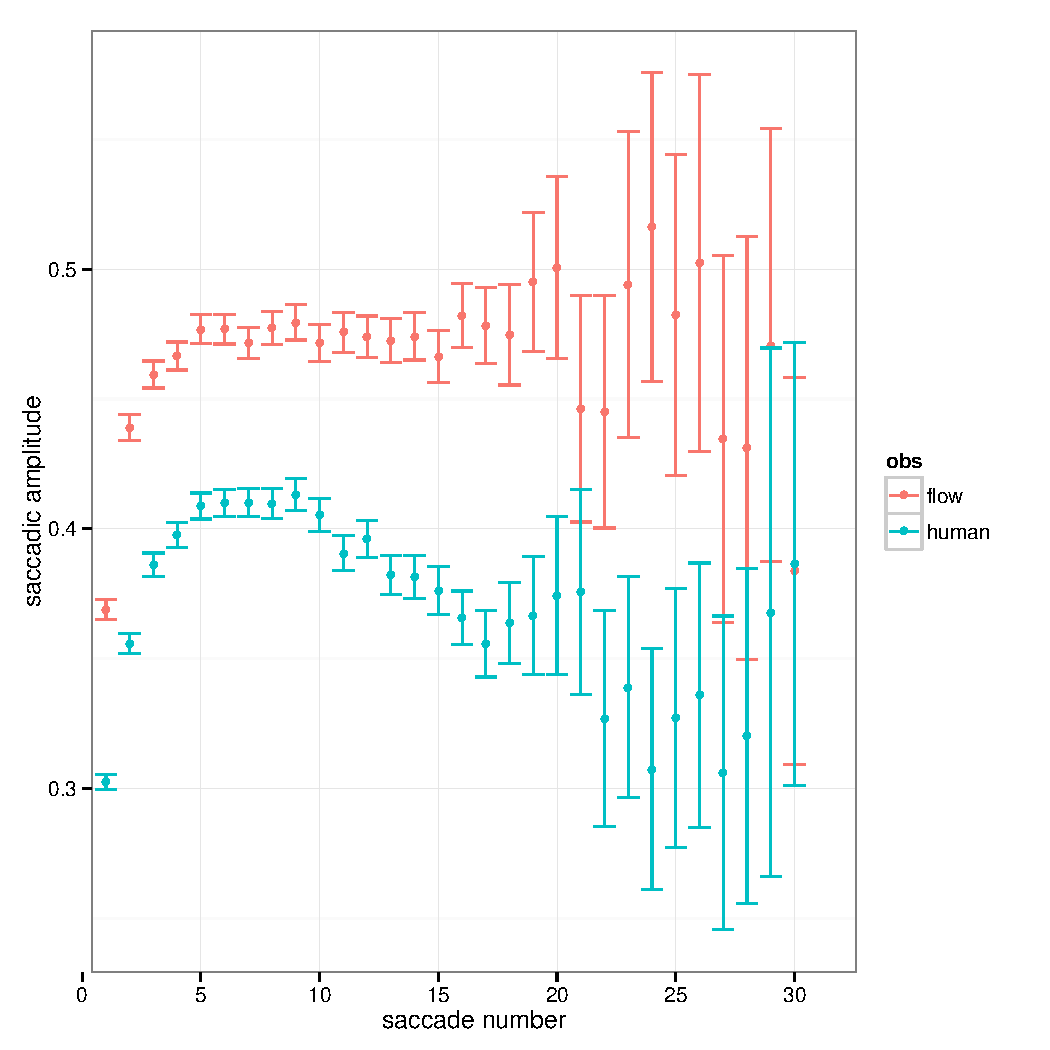
\includegraphics[width=3.8cm]{../scripts/coarse2fine/figs/saccAmpOverTimeFlow}}
\caption[]{\textit{blue}: human, \textit{red}: central bias, \textit{green}: saccadic flow. \textit{top row}: Comparison of $x$ and $y$ fixation positions between human fixations and synthetic points generated from the central bias and flow model. \textit{bottom row}: We can see that the flow model consistently makes saccades with a slightly larger amplitude than human observers. Distances are expressed relative to the width of the image. Best fit line in (d) fitted with loess regression. All distances are given in normalised units in which the width of an image is 2 (see Section \ref{sec:modellingMethods}).}
\label{fig:flowHumanComp}
\end{figure}


\subsection{Discussion}

We have demonstrated different ways biases such as saccadic flow and the central bias can be used in eye movement research. They can be used as a prior on the probability of making saccades to different regions of the image, allowing us to then more clearly visualise the image-dependant behaviour. We have also shown that the likelihoods of fixations under the bias models are related to features such as salience. The interpretation of visual salience as a predictive model of fixation selection can therefore be informed by considering how likely a saccade is to be generated by these models. Finally, we can also use the bias distributions to generate synthetic data that can be used as control points in ROC analysis, and to explore which aspects of human saccadic dynamics are not captured by the simple flow model. 
